\documentclass[../main.tex]{subfiles}

\begin{document}

The system was fully tested only on linux environment, for which the following instructions will be valid, though it should run on all major platforms with proper adjustments. To evaluate all components of this prototype, at least these software packages must be installed and working on the system in use:

\begin{itemize}
	\item Node JS (11.6.0)
	\item npm (6.5.0)
	\item Flutter (1.0.0 - rev. 5391447fae)
	\item Dart (2.1.0)
	\item JDK/OpenJDK 8
	\item Android Studio or Intellij Idea - for the wearable application
	\item adb tool
\end{itemize}

In parenheses is indicated the version used in development. Following are the steps to launch the various components:

\subsection{Backend server}

\begin{itemize}
	\item Eventually import the project ITD/TrackMeServer in Android Studio / Intellij Idea (not required).
	\item Navigate to ITD/TrackMeServer and run "npm install" to download the required dependencies (defined in package.json).
	\item Edit the common/config.json file with address and port on which each component should listen for incoming connections.
	\item Edit the common/config.json file setting to "true" the postgres.useHeroku variable to use an already set up DBMS. It is though advised to use a local DBMS connection (PostgresQL) if possible, since it allows to browse the data in the database. In this case, set the useHeroku variable to "false" and properly set the other three variables.
	\item Run the components by executing \newline "node DatabaseServer/DatabaseServer.js \& \newline node ApplicationServerMobileClient/ApplicationServerMobileClient.js \& \newline node ApplicationServerData4Help/ApplicationServerData4Help.js \& \newline node WebServer/WebServer.js \&" \newline or by launching them from the IDE.
\end{itemize}

Note that the working directory for the processes must be ITD/TrackMeServer, otherwise some necessary files won't be found. Also, each module can be launched on a different directory, or a different host, as long as the "common" and "node\textunderscore modules" directories are present along the component's one.

Also, every variable defined in config.json can be overridden with environment variables. The structure of such variables is equal to the ones in the configuration file, with the following differences: all character are uppercase, and to address a sub-variable, use the underscore. For example, to temporarily use the heroku DBMS, one could launch the DatabaseServer like this:\newline
POSTGRES\textunderscore USEHEROKU=true node DatabaseServer/DatabaseServer.js

\subsubsection{Automated tests}
After the Mocha and Chai have been installed, the tests defined in test/test.js can be run by navigating to ITD/TrackMeServer and running "./node\textunderscore modules/mocha/bin/mocha test/test.js", or by launching a proper Mocha run configuration from the IDE. Note that these tests require the three major components of the backend server to be running; also, after the tests have been run once, the database needs to be reset, otherwise some of them will fail.

\subsubsection{Support files for evaluation}

Inside the "support" directory there are some files useful for evaluating the project, as stated in chapter 4. To launch the python scripts, just run "python3 \textit{path-to-py-file}". Note that they also need the common/config.json file to be in the working directory.

A Postman configuration, that was also used for testing, is also supplied. To import it, just launch Postman, then click import and open postman.json file. The following functions are defined: \newline

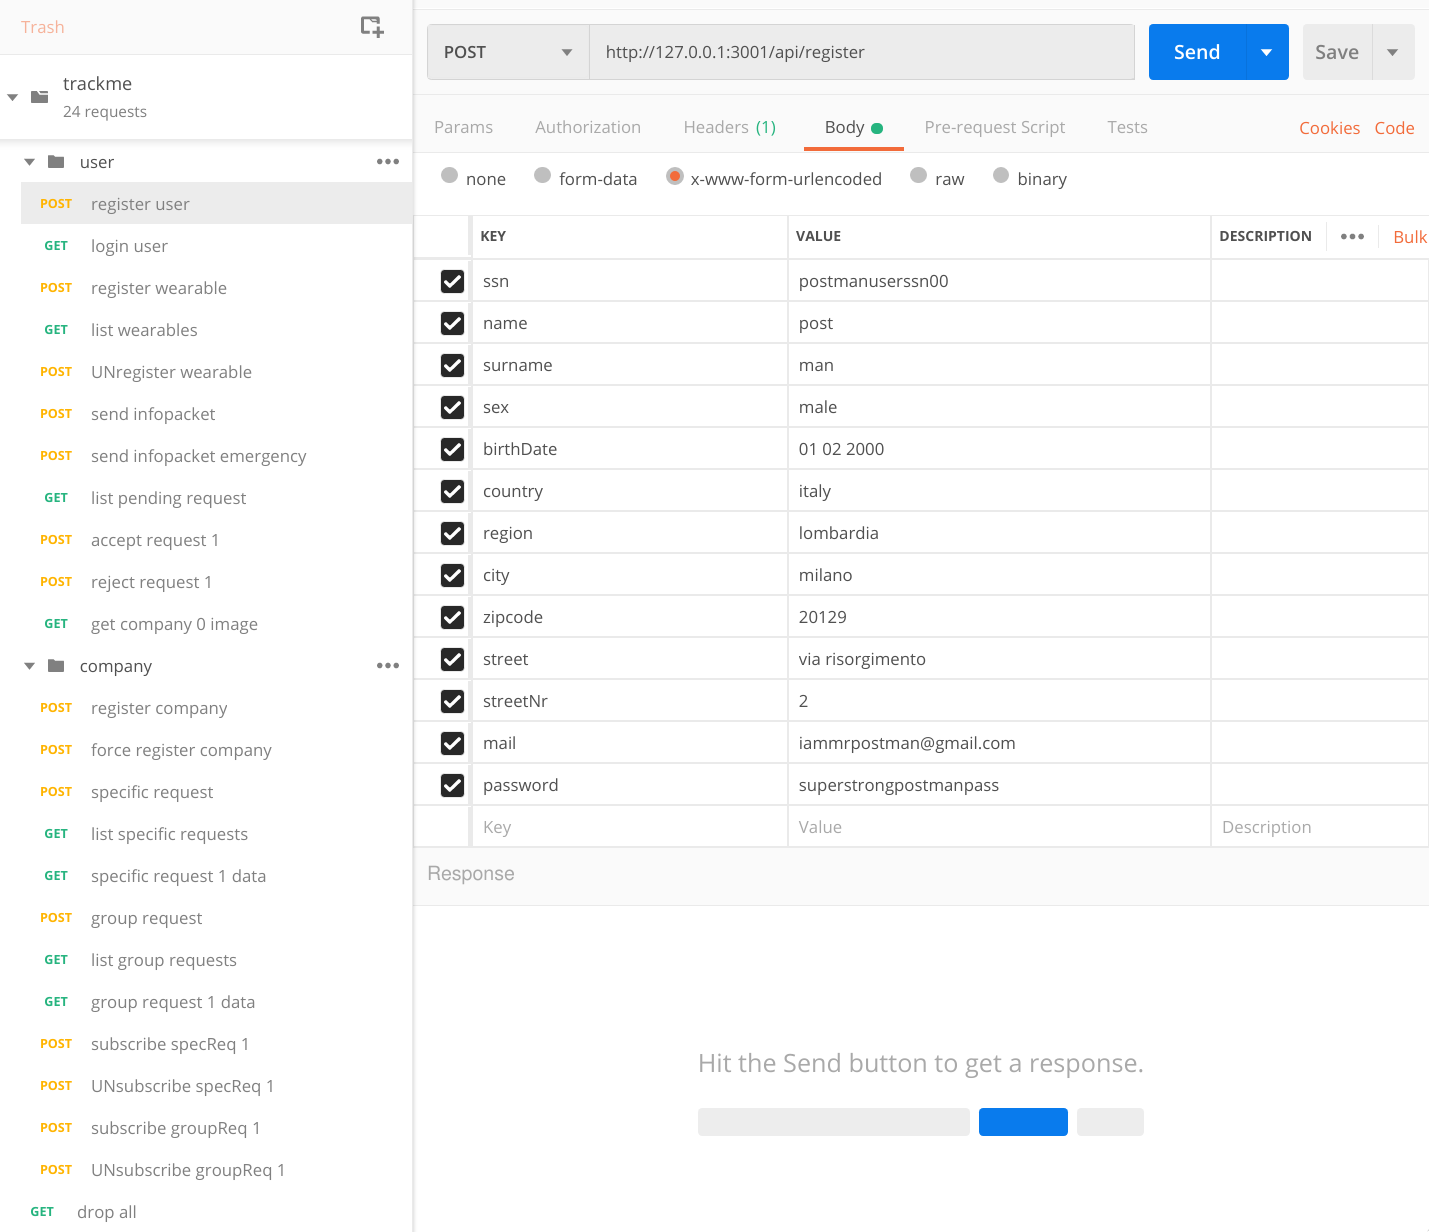
\includegraphics[width = \linewidth ]{images/postman_screen.png}

\subsubsection{Email credentials}
The mail box where registration requests are sent can be checked using the following credentials:
\begin{description}
	\item email: wtrackme@gmail.com
	\item password: Data4.Help
\end{description}


\subsection{MobileApp TrackmeMobile}

\begin{itemize}
	\item Eventually import the project ITD/MobileApp/TrackmeMobile/trackmemobile into Android Studio / Intellij Idea (not required).
	\item Edit the file trackmemobile/lib/ProfileManager/network.dart and set the \textunderscore url variable with the ip address on which the Application Server Mobile Client component will be reachable (this won't be 127.0.0.1!). At the same way edit the variable basicUrl in trackmemobile/android/app/src/main/java/com/trackme/trackmemobile/InfoPacketHandler.java.
	\item Assuming Flutter SDK, Android SDK and Dart are installed, and Flutter's bin directory is in PATH environment variable, navigate to ITD/MobileApp/TrackmeMobile/trackmemobile.
	\item Run "flutter build apk --debug"; this will generate the apk in build/app/outputs/apk/debug/app-debug.apk
	\item Install the apk on the device (eg. with "adb install \textit{path-to-apk}") and run it.
\end{itemize}

Alternatively one can build and install the apk from the IDE.

\subsection{MobileApp TrackmeWear}

\begin{itemize}
	\item Import the project ITD/MobileApp/TrackmeWear into the IDE (required!).
	\item Create an Android App run configuration setting the Module field to "app", if does not exist.
	\item Launch an Android Wear virtual device.
	\item Run the app on the virtual device.
	\item Run in a terminal "adb -d forward tcp:5601 tcp:5601", to allow the wearable to communicate with the Android phone, and connect the smartphone to adb. Make sure it is listed as "device" when running "adb devices", not as "unauthorized".
	\item Download, install and run the Wear OS application from the play store on your Android phone, and pair it with the emulator.
	\item Run the wearable application on the emulator.
\end{itemize}

Note that the wearable device emulator won't connect with a smartphone emulator, so a real smartphone and the wearable emulator must be used.

\end{document}
